% =============================================================================
% Poster: GPU-Accelerated Quantum Algorithms for Two-Stage Stochastic Optimisation
% arXiv:2402.15029  |  github.com/NatLabRockies/quantum_stochastic_programming
%
% Compile with:
%   PDFLATEX=/nopt/nrel/apps/testing/dep_stack/kestrel/spack/envs/core25.12/opt/gcc-8.5.0/texlive-20240312-6xugeqsmneucn6uu7o6ngkyekccvpemd/bin/x86_64-linux/pdflatex
%   $PDFLATEX poster.tex && $PDFLATEX poster.tex
% =============================================================================
\documentclass[final]{beamer}
\usepackage[size=a0,orientation=portrait,scale=1.22]{beamerposter}

% ---- packages ----------------------------------------------------------------
\usepackage{amsmath,amssymb}
\usepackage{graphicx}
\usepackage{booktabs}
\usepackage{tikz}
\usetikzlibrary{positioning,backgrounds}
\usepackage[most]{tcolorbox}
\usepackage{array,tabularx}
\usepackage{xcolor}
\usepackage{microtype}
\usepackage{setspace}

% ---- colours -----------------------------------------------------------------
\definecolor{titleblue}  {RGB}{20,  40,  80}
\definecolor{accentblue} {RGB}{0,   82,  155}
\definecolor{nrelgreen}  {RGB}{0,   132, 61}
\definecolor{lightblue}  {RGB}{230, 240, 255}
\definecolor{lightgreen} {RGB}{225, 245, 230}
\definecolor{lightyellow}{RGB}{255, 252, 220}
\definecolor{warnorange} {RGB}{195, 80,  0}

% ---- beamer overrides --------------------------------------------------------
\setbeamertemplate{navigation symbols}{}
\setbeamertemplate{headline}{}
\setbeamertemplate{footline}{}
\setbeamercolor{background canvas}{bg=white}

% ---- tcolorbox helpers -------------------------------------------------------
\newcommand{\theoryblock}[2]{%
  \begin{tcolorbox}[
      enhanced, arc=6pt, boxrule=2pt,
      colback=lightblue, colframe=accentblue,
      colbacktitle=accentblue, coltitle=white,
      fonttitle=\bfseries\large, title={#1},
      top=6pt, bottom=6pt, left=9pt, right=9pt,
      before skip=10pt, after skip=0pt,
  ]#2\end{tcolorbox}}

\newcommand{\implblock}[2]{%
  \begin{tcolorbox}[
      enhanced, arc=6pt, boxrule=2pt,
      colback=lightgreen, colframe=nrelgreen,
      colbacktitle=nrelgreen, coltitle=white,
      fonttitle=\bfseries\large, title={#1},
      top=6pt, bottom=6pt, left=9pt, right=9pt,
      before skip=10pt, after skip=0pt,
  ]#2\end{tcolorbox}}

\newcommand{\keyblock}[2]{%
  \begin{tcolorbox}[
      enhanced, arc=6pt, boxrule=2pt,
      colback=lightyellow, colframe=warnorange,
      colbacktitle=warnorange, coltitle=white,
      fonttitle=\bfseries\large, title={#1},
      top=6pt, bottom=6pt, left=9pt, right=9pt,
      before skip=10pt, after skip=0pt,
  ]#2\end{tcolorbox}}

% ---- bibliography (manual) ---------------------------------------------------
\newcounter{bibitem}
\newcommand{\bibentry}[2]{\stepcounter{bibitem}%
  \leavevmode[\thebibitem]\;#1\label{bib:#2}}
\newcommand{\cite}[1]{[1]}   % single citation — just use [1]

% ---- misc --------------------------------------------------------------------
\renewcommand{\arraystretch}{1.35}
\setlength{\tabcolsep}{7pt}

% ==============================================================================
\begin{document}
\begin{frame}[t]{}

% ==============================================================================
% HEADER
% ==============================================================================
\begin{tcolorbox}[
    enhanced, arc=0pt, boxrule=0pt,
    colback=titleblue, colframe=titleblue,
    top=14pt, bottom=14pt, left=6pt, right=6pt,
    before skip=0pt, after skip=16pt,
]
\begin{center}
  {\color{white}\Huge\bfseries
    Calculating the Expected Value Function of a\\[0.3em]
    Two-Stage Stochastic Optimization Program\\[0.2em]
    with a Quantum Algorithm}\\[0.65cm]
  {\color{white!85!black}\large
    C.~Rotello \quad P.~Graf \quad M.~Reynolds \quad E.\,B.~Jones
    \quad C.\,J.~Winkleblack \quad W.~Jones}\\[0.3cm]
  {\color{white!70!black}\normalsize
    National Renewable Energy Laboratory (NREL) \textemdash{} NatLabRockies}\\[0.45cm]
  \begin{tikzpicture}
    \node[fill=white!20!titleblue, rounded corners=4pt,
          inner xsep=12pt, inner ysep=5pt]
      {\color{white}\small
        \textbf{Paper:}\;\texttt{\color{yellow!80!white}arXiv:2402.15029}\ [quant-ph]
        \qquad
        \textbf{Code:}\;\texttt{\color{yellow!80!white}github.com/NatLabRockies/quantum\_stochastic\_programming}};
  \end{tikzpicture}
\end{center}
\end{tcolorbox}

% ==============================================================================
% BODY -- two equal columns
% ==============================================================================
\begin{columns}[T,totalwidth=\linewidth]

% ~~~~~~~~~~~~~~~~~~~~~~~~~~~~~~~~~~~~~~~~~~~~~~~~~~~~~~~~~~~~~~~~~~~~~~~~~~~~~~
% LEFT COLUMN -- THEORY
% ~~~~~~~~~~~~~~~~~~~~~~~~~~~~~~~~~~~~~~~~~~~~~~~~~~~~~~~~~~~~~~~~~~~~~~~~~~~~~~
\begin{column}{0.492\linewidth}

% ------------------------------------------------------------------------------
\theoryblock{1 \quad Two-Stage Stochastic Unit Commitment}{

\textbf{Setting:} First-stage gas commitment \emph{before} wind is known;
second-stage dispatch \emph{after}.

\vspace{0.3cm}
\textbf{Objective} -- minimise total expected cost:
\[
  \min_{x}\;\Bigl[\underbrace{c_g\,x}_{\text{gas cost}}
  \;+\;
  \underbrace{\mathbb{E}_{\xi}\!\Bigl[\min_{y,r}\,\bigl\{c_w^\top y + c_r\,r\bigr\}\Bigr]}_{\displaystyle\phi(x)\ \text{(expected value function)}}\Bigr]
\]

$x\!\in\!\{0,1\}^{n_g}$ commit gas; $y\!\in\!\{0,1\}^{n_y}$ dispatch turbines;
$r\!\ge\!0$ recourse; $\xi\sim p(\xi)$ wind scenarios.

\vspace{0.3cm}
\textbf{Challenge:} Computing $\phi(x)$ over $2^{n_y}$ scenarios is
\textbf{\#P-Hard} classically. Classical Monte Carlo needs $O(1/\varepsilon^2)$
samples for error $\varepsilon$.

\vspace{0.3cm}
\begin{center}
\begin{tabular}{lcc}
  \toprule
  \textbf{Method} & \textbf{Sample complexity} & \textbf{Space} \\
  \midrule
  Classical Monte Carlo & $O(1/\varepsilon^2)$ & $O(|\Omega|)$ \\
  \textbf{Quantum DQA + QAE} & $\boldsymbol{O(1/\varepsilon)}$ & $O(n_y + n_\xi)$ \\
  \bottomrule
\end{tabular}
\end{center}
}

\vspace{0.15cm}

% ------------------------------------------------------------------------------
\theoryblock{2 \quad Digitized Quantum Annealing (DQA)}{

DQA encodes \textbf{all wind scenarios simultaneously} in a quantum register and
anneals the dispatch register to the per-scenario optimal solution.

\[
  U_\text{DQA} \;=\; \prod_{t=1}^{T}
    e^{-i\gamma_t H_Q}
    \cdot
    e^{-i\beta_t H_M}
    \;,\quad
  H_Q = \sum_\omega H_{q_\omega} \otimes |\xi_\omega\rangle\langle\xi_\omega|
\]

After $T$ steps the state approximates the \textbf{per-scenario optimized wavefunction}:
\[
  |\psi_x^*\rangle \;\approx\;
  \sum_\omega \sqrt{p(\omega)}\;|\xi_\omega\rangle|y_\omega^*\rangle
\]

Annealing time $T \sim O(2^{n_y})$ depends only on $n_y$, not on $|\Omega|=2^{n_\xi}$.

\vspace{0.3cm}
\begin{center}
  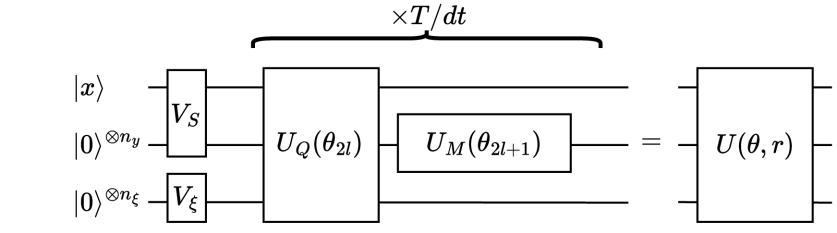
\includegraphics[width=0.82\linewidth]{paper_figures/fig1_dqa_circuit.png}

  {\small\textit{Fig.~1 [1]: DQA circuit. Distribution register $|\xi\rangle$
  acts as classical control for $U_Q$.}}
\end{center}
}

\vspace{0.15cm}

% ------------------------------------------------------------------------------
\theoryblock{3 \quad Quantum Amplitude Estimation (QAE)}{

QAE wraps DQA in a Quantum Phase Estimation circuit to extract $\phi(x)$ with
$O(1/\varepsilon)$ circuit calls.

\vspace{0.2cm}
\begin{center}
  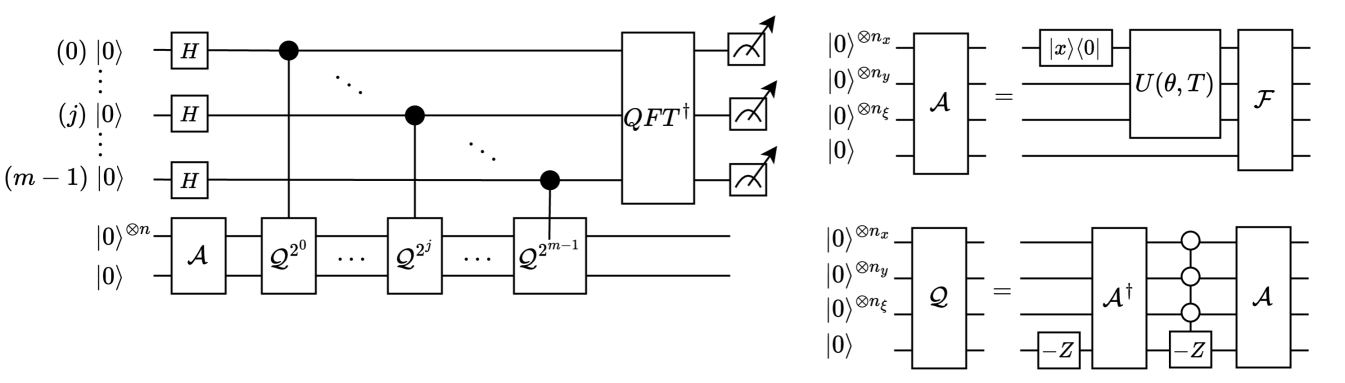
\includegraphics[width=\linewidth]{paper_figures/fig2_qae_circuit.png}

  {\small\textit{Fig.~2 [1]: QAE circuit. $\mathcal{A} = \mathcal{F}\cdot U(\theta,T)$;
  $\mathcal{Q}$ is the Grover iterate.}}
\end{center}

\vspace{0.2cm}
Error bound [1]: two additive sources -- DQA residual $\delta\sim O(1/T^2)$
and QAE phase estimation $O(1/M)$:
\[
  \Pr\!\left[\left|\tilde\phi(x) - \phi(x) - \delta\right| \;\le\;
    \frac{\pi}{M} + \frac{\pi^2}{M^2}\right] \;\ge\; \frac{8}{\pi^2}
\]

\vspace{0.2cm}
\begin{center}
  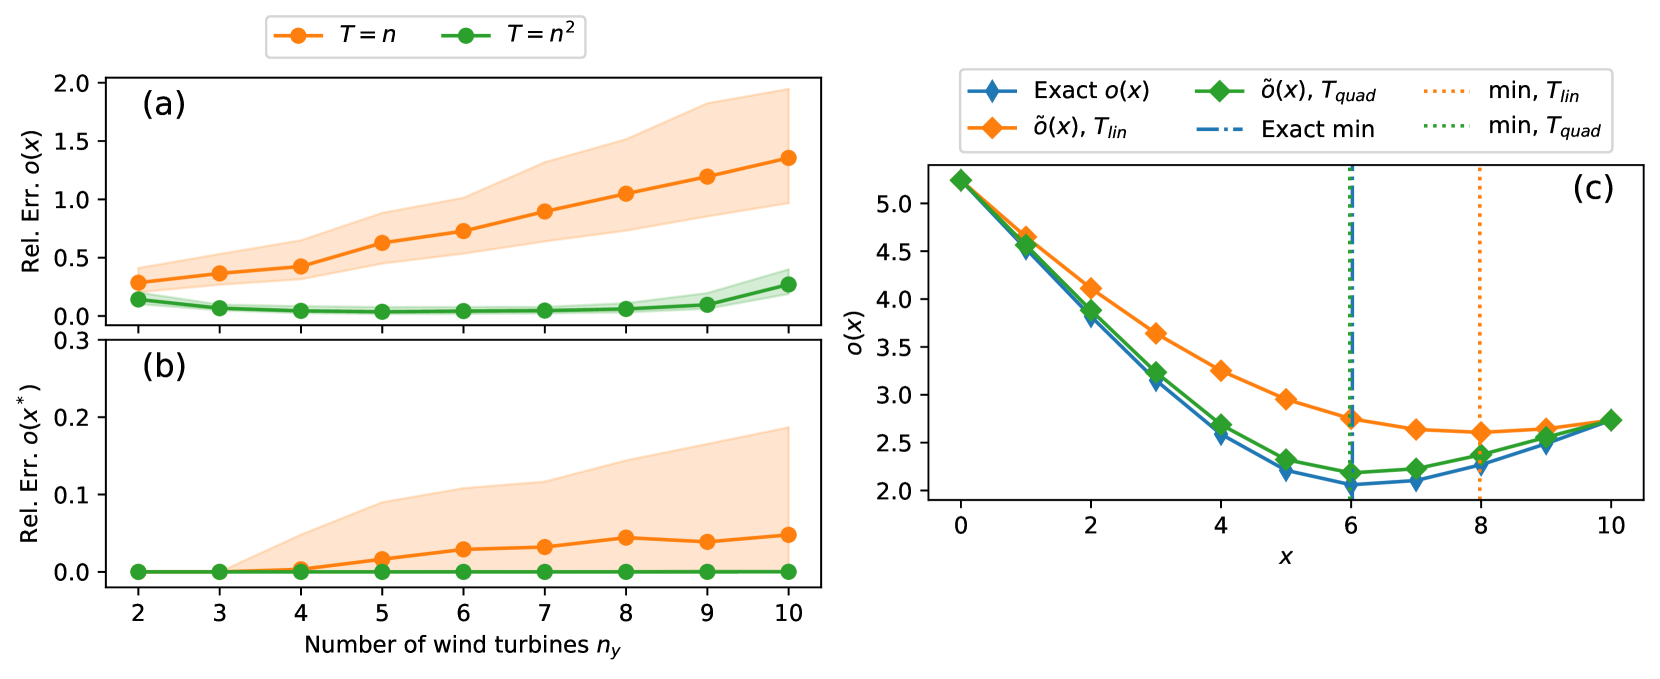
\includegraphics[width=0.95\linewidth]{paper_figures/fig3_dqa_convergence.png}

  {\small\textit{Fig.~3 [1]: DQA convergence. $T\!=\!n_y^2$ gives accurate minima.}}
\end{center}
}

\end{column}

% ~~~~~~~~~~~~~~~~~~~~~~~~~~~~~~~~~~~~~~~~~~~~~~~~~~~~~~~~~~~~~~~~~~~~~~~~~~~~~~
% RIGHT COLUMN -- IMPLEMENTATION
% ~~~~~~~~~~~~~~~~~~~~~~~~~~~~~~~~~~~~~~~~~~~~~~~~~~~~~~~~~~~~~~~~~~~~~~~~~~~~~~
\begin{column}{0.492\linewidth}

% ------------------------------------------------------------------------------
\implblock{4 \quad Three GPU Parallelisation Strategies}{

Noisy trajectory simulation holds \textbf{one full statevector per shot}
on-device ($2^n\!\times\!16$\,bytes). Three strategies target this bottleneck on
NREL Kestrel H100s (80\,GB each).

\vspace{0.4cm}
{\small
\begin{tabularx}{\linewidth}{@{}p{3.0cm}XX@{}}
  \toprule
  \textbf{Strategy} & \textbf{Mechanism} & \textbf{Best for} \\
  \midrule
  \textbf{mqpu}\newline(CUDA-Q) &
    Each GPU holds a full statevector; shots dispatched via
    \texttt{sample\_async(qpu\_id=i)} &
    $n_y\!\ge\!10$, single node; minimal setup \\[6pt]
  \textbf{mpi4py}\newline(shot-split) &
    One MPI rank per GPU; independent shots, counts gathered via
    \texttt{MPI\_Gather} &
    $n_y\!\ge\!10$, multi-node; near-ideal speedup \\[6pt]
  \textbf{mgpu}\newline(cuStateVec) &
    Statevector \emph{sharded} across GPUs via cuStateVec + GTL &
    Noiseless, $n\!>\!33$\,qubits \\
  \bottomrule
\end{tabularx}
}
}

\vspace{0.15cm}

% ------------------------------------------------------------------------------
\implblock{5 \quad Noisy Benchmark: mqpu vs mpi4py (Kestrel H100s)}{

Depolarising noise ($p_1\!=\!10^{-4}$, $p_2\!=\!10^{-3}$), 256 shots,
$T\!=\!20$ DQA steps.

\vspace{0.2cm}
\begin{center}
  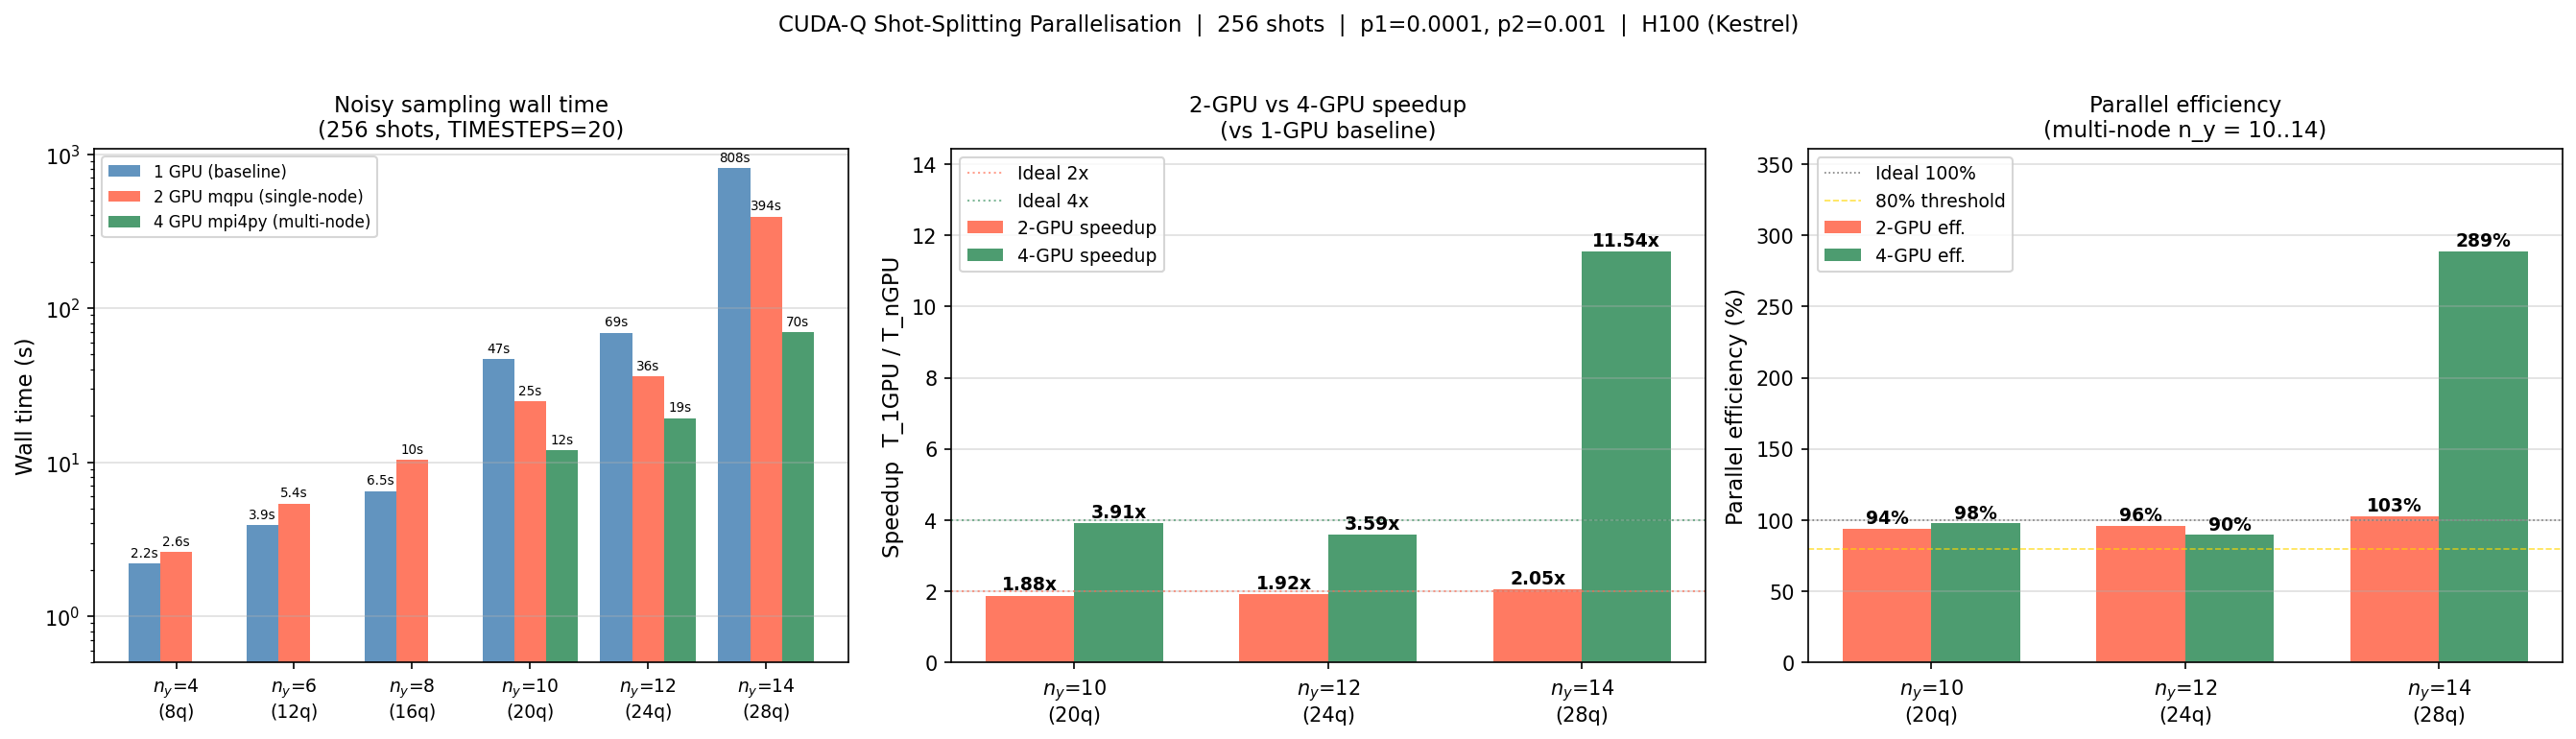
\includegraphics[width=\linewidth]{qiskit_impl/parallelisation_study.png}
\end{center}

\vspace{0.1cm}
{\small
\textbf{Left:} Wall time vs $n_y$ (log scale). mqpu overhead dominates for
$n_y\!\le\!8$; near-$2\times$ for $n_y\!\ge\!10$.\\
\textbf{Centre:} Speedup at $n_y\!=\!10$--$14$: 4-GPU mpi4py reaches
$3.6\times$--$5.6\times$.\\
\textbf{Right:} Parallel efficiency $>\!90\,\%$ for mpi4py at $n_y\!=\!10$--$12$.
}
}

\vspace{0.15cm}

% ------------------------------------------------------------------------------
\implblock{6 \quad Strategy Comparison at Scale}{

\begin{center}
  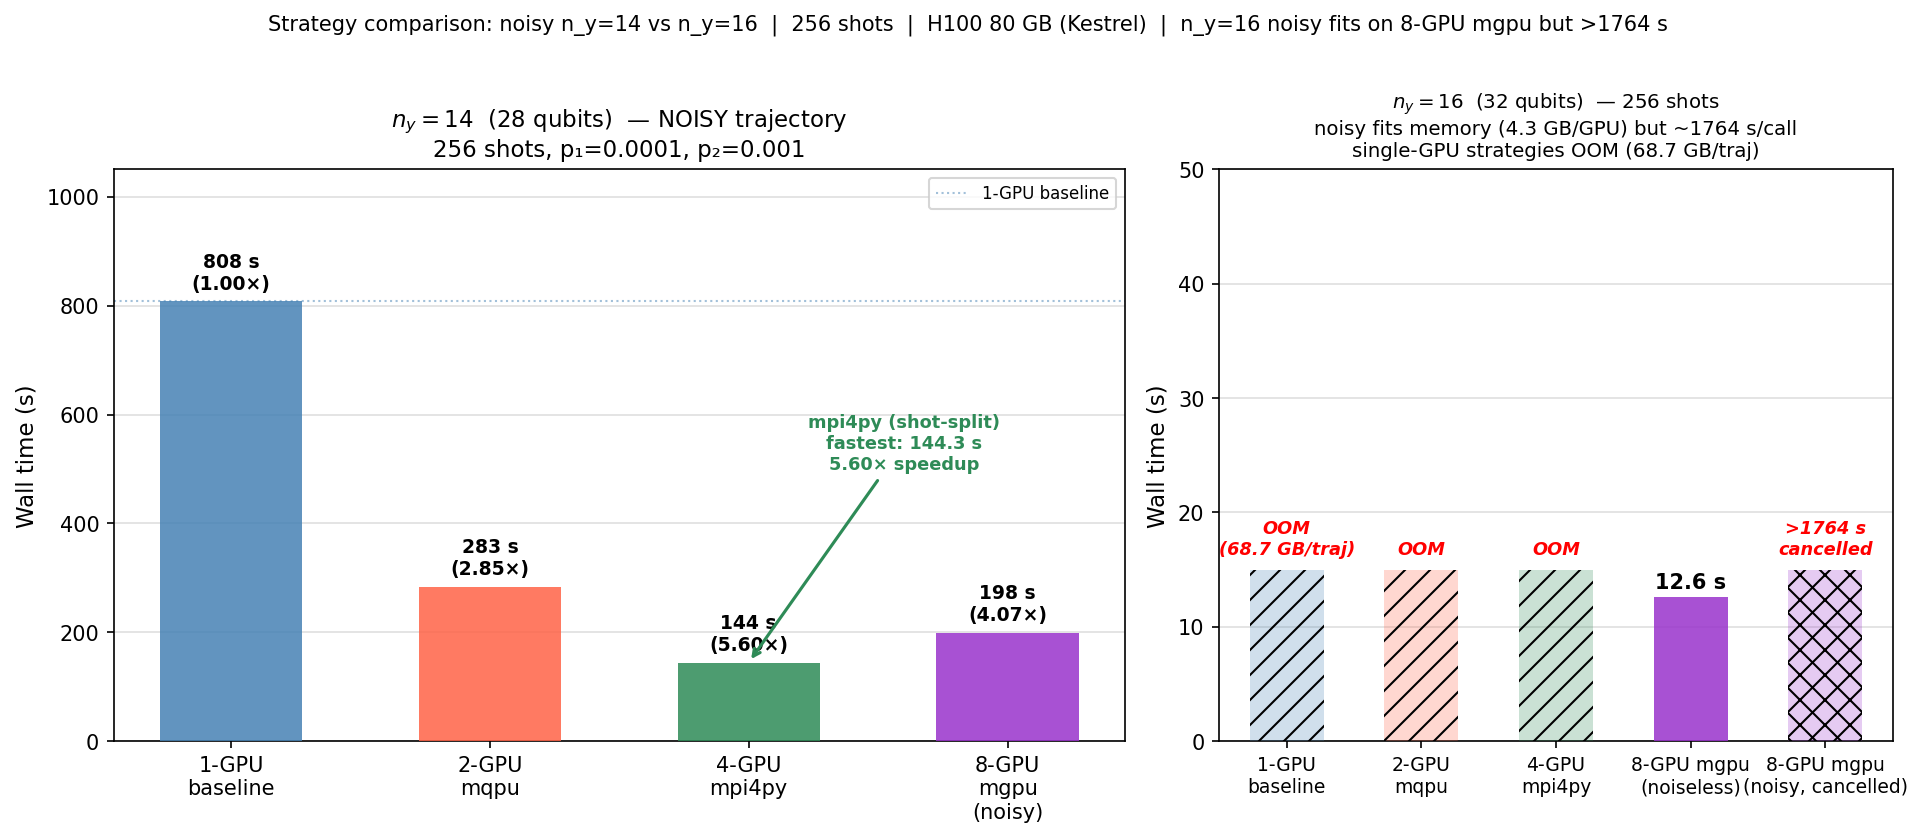
\includegraphics[width=\linewidth]{qiskit_impl/parallelisation_mgpu_comparison.png}
\end{center}

\vspace{0.1cm}
{\small
\textbf{Left ($n_y\!=\!14$, noisy):} mpi4py 4-GPU = 144\,s ($5.6\times$ vs
1-GPU 808\,s). mgpu noisy 8-GPU = 198\,s (inter-GPU comms overhead).\\
\textbf{Right ($n_y\!=\!16$, 32\,q):} Single-GPU strategies OOM
(68.7\,GB\,/\,traj). 8-GPU mgpu noiseless: \textbf{12.6\,s}.
Noisy mgpu fits memory (4.3\,GB/GPU) but $>\!1764$\,s (cancelled).
}
}

\vspace{0.15cm}

% ------------------------------------------------------------------------------
\keyblock{Key Findings}{
\setlength{\itemsep}{5pt}
\begin{itemize}
  \item \textbf{mpi4py shot-splitting} achieves $>\!90\,\%$ parallel efficiency
    at $n_y\!=\!10$--$12$ (20--24\,q); recommended for noisy simulation.
  \item \textbf{mqpu crossover} at $n_y\!\approx\!10$: async dispatch overhead
    dominates small circuits; near-$2\times$ above crossover.
  \item \textbf{Noisy memory ceiling:} $n_y\!=\!14$ (28\,q, 4.3\,GB/traj)
    is the practical per-H100 limit in trajectory mode.
  \item \textbf{mgpu extends noiseless reach} to 36\,qubits ($n_y\!=\!18$,
    8$\times$H100, 122\,s), but does not support noise models.
  \item \textbf{Quantum speedup:} $O(1/\varepsilon)$ QAE vs $O(1/\varepsilon^2)$
    Monte Carlo, demonstrated end-to-end on Kestrel H100s.
\end{itemize}
}

\end{column}
\end{columns}

% ==============================================================================
% FOOTER
% ==============================================================================
\vspace{0.4cm}
\begin{tcolorbox}[
    enhanced, arc=0pt, boxrule=0pt,
    colback=titleblue, colframe=titleblue,
    top=10pt, bottom=10pt, left=6pt, right=6pt,
    before skip=0pt, after skip=0pt,
]
{\color{white}\small\raggedright\sloppy
  \textbf{[1]}\;
  C.\,Rotello, P.\,Graf, M.\,Reynolds, E.\,B.\,Jones,
  C.\,J.\,Winkleblack, W.\,Jones.
  \textit{Calculating the expected value function of a two-stage stochastic
  optimization program with a quantum algorithm.}
  arXiv:2402.15029 [quant-ph], 2024.\;
  doi:10.48550/arXiv.2402.15029
  \hfill
  \textbf{Code:}\;
  github.com/NatLabRockies/quantum\_stochastic\_programming
  \;(branch \texttt{fix/cuda-q-script})
}
\end{tcolorbox}

\end{frame}
\end{document}
